
\subsubsection*{Introduction}
The Brute Force algorithm for d-partite matching works by exhaustively searching through all possible subsets of edges within the graph, identifying the largest subset that forms a valid matching. This approach guarantees that the maximum matching is found, as it explores every possible combination of edges. However, it is computationally intensive and becomes increasingly impractical for large graphs due to the sheer number of edge subsets to evaluate.

\subsubsection*{Algorithm:}
The Brute Force algorithm follows these steps to identify the maximum matching:

\begin{enumerate}

    \item \textbf{Iterate Through All Edge Subsets}: For every possible subset of edges (from size \( n \) to 1):
    \begin{itemize}
        \item \textbf{Check for Valid Matching}: Determine if the current subset of edges forms a valid matching by ensuring no two edges in the subset share a common vertex.
        \item \textbf{Stop at the first Maximum Matching}: If the current subset forms a valid matching then, that is the solution of the problem.
    \end{itemize}
    \item \textbf{Return the Largest Valid Subset}: Examine all subsets from $n$ to 1 until the first matching is found, and return that subset which forms a valid matching.
\end{enumerate}

This exhaustive search approach ensures that the largest possible matching is found, making it an accurate but computationally expensive method.

\subsubsection*{Checking if an Edge is Valid in the Matching Set:}
To determine whether a subset of edges forms a valid matching, each edge must satisfy the requirement that no two edges in the matching share a vertex. This criterion can be tracked using a two-dimensional array, \texttt{d\_table}, which helps ensure that no vertices are repeated across different edges in the subset:

\begin{itemize}
    \item \textbf{Criteria for a Valid Edge}: No two edges in the matching can share a vertex.
    \item \textbf{Tracking Shared Vertices}: Initialize \texttt{d\_table} as a list of lists: \texttt{d\_table = [ [], [], [], ... ]} with \( d \) empty lists.
    \begin{itemize}
        \item Each list \texttt{d\_table[i]} represents the vertices in the \( i \)th dimension or column of the d-partite graph.
        \item As edges are evaluated, \texttt{d\_table} keeps track of vertices included in each dimension to avoid overlaps.
    \end{itemize}
\end{itemize}

This approach ensures that each subset is correctly validated, though it adds to the computational overhead due to constant updates and checks on the \texttt{d\_table}.

\newpage

\subsection*{Brute Force Solver Pseudocode}

\begin{algorithm}
\caption{Brute Force Solver}
\begin{algorithmic}[1]
\STATE \textbf{Input:} Graph $G$ with dimensions $d$, vertices $n$, edges $m$, and edge set $E$
\STATE \textbf{Output:} Maximum matching subset of edges

\FOR{$r \gets n$ \textbf{down to} $1$}
    \FOR{each subset $\textit{edge\_comb}$ of size $r$ from $E$}
        \IF{$\textit{is\_valid\_combination}(\textit{edge\_comb}, d)$}
            \RETURN $\textit{edge\_comb}$ \hfill // Return valid matching immediately
        \ENDIF
    \ENDFOR
\ENDFOR
\RETURN $[]$ \hfill // Return empty list if no matching found
\end{algorithmic}
\end{algorithm}

% \subsection*{is\_valid\_combination Function Pseudocode}

\begin{algorithm}
\caption{is\_valid\_combination}
\begin{algorithmic}
\STATE \textbf{Input:} Edge combination $\textit{edge\_comb}$, dimension $d$
\STATE Initialize $d\_table \gets [\{\}, \{\}, \dots, \{\}]$ (an array of $d$ empty sets)
\FOR{each edge $e$ in $\textit{edge\_comb}$}
    \FOR{$i \gets 1$ \textbf{to} $d$}
        \IF{$e[i]$ is in $d\_table[i]$}
            \RETURN \textbf{False} \hfill // Invalid if vertex is already used
        \ENDIF
        \STATE Add $e[i]$ to $d\_table[i]$
    \ENDFOR
\ENDFOR
\RETURN \textbf{True} \hfill // Valid matching if no vertices overlap
\end{algorithmic}
\end{algorithm}



\subsubsection*{Example:}


Consider a simple example where:
\[
d = 2, \quad n = 3, \quad m = 4, \quad E = \{ [1, 1], [2, 1], [3, 2], [3, 3] \}
\]

\begin{center}
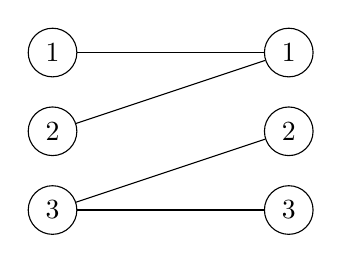
\begin{tikzpicture}
    % Define nodes for two sets
    \node[circle, draw] (A1) at (0, 1) {1};
    \node[circle, draw] (A2) at (0, 0) {2};
    \node[circle, draw] (A3) at (0, -1) {3};

    \node[circle, draw] (B1) at (3, 1) {1};
    \node[circle, draw] (B2) at (3, 0) {2};
    \node[circle, draw] (B3) at (3, -1) {3};

    % Draw edges
    \draw (A1) -- (B1) node[midway, above] {};
    \draw (A2) -- (B1) node[midway, above] {};
    \draw (A3) -- (B2) node[midway, above] {};
    \draw (A3) -- (B3) node[midway, above] {};

\end{tikzpicture}
\end{center}
\begin{center}
    \textbf{Figure:} The Graph representation of the problem above
\end{center}

The brute force algorithm examines all possible subsets of edges from size \( n \) down to 1 and picks the first valid matching.


\paragraph{All Possible Subsets of edges:}
\begin{itemize}
    \item Size 1: \([1, 1], [2, 1], [3, 2], [3, 3]\)
    \item Size 2: \(\{[1, 1], [2, 1]\}, \{[1, 1], [3, 2]\}, \{[1, 1], [3, 3]\}, \{[2, 1], [3, 2]\}, \{[2, 1], [3, 3]\}, \{[3, 2], [3, 3]\}\)
    \item Size 3: \(\{[1, 1], [2, 1], [3, 2]\}, \{[1, 1], [2, 1], [3, 3]\}, \{[1, 1], [3, 2], [3, 3]\}, \{[2, 1], [3, 2], [3, 3]\}\)
\end{itemize}

Initially, the algorithm will iterate through all subsets of size $n=3$ to see if any subset forms a valid matching. In this example, no subset of size 3 forms a valid matching, thus, the algorithm will then check for subsets of size $n-1 = 2$. The subset $\{[1, 1], [3, 2]\}$ forms a valid matching. Hence, it will return this subset as the solution to this problem.


\begin{center}
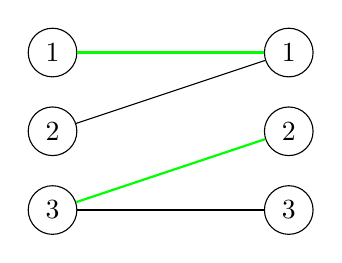
\begin{tikzpicture}
    % Define nodes for two sets
    \node[circle, draw] (A1) at (0, 1) {1};
    \node[circle, draw] (A2) at (0, 0) {2};
    \node[circle, draw] (A3) at (0, -1) {3};

    \node[circle, draw] (B1) at (3, 1) {1};
    \node[circle, draw] (B2) at (3, 0) {2};
    \node[circle, draw] (B3) at (3, -1) {3};

    % Draw edges
    \draw[green, thick] (A1) -- (B1) node[midway, above] {};
    \draw (A2) -- (B1) node[midway, above] {};
    \draw[green, thick] (A3) -- (B2) node[midway, above] {};
    \draw (A3) -- (B3) node[midway, above] {};

\end{tikzpicture}

\end{center}
\begin{center}
    \textbf{Figure:} Solution to the above problem, with $Matching =$ \(\{[1, 1], [3, 2]\}\) highlighted in green.
\end{center}


This example demonstrates how the brute force algorithm systematically examines each subset of edges to identify a valid matching.

\subsubsection*{Complexity:}
The complexity of this algorithm can be estimated through the choices made by the algorithm. The maximum matching size can be up to $n$, which is given by the set of edges that form a valid matching. Thus, in the worst case, the algorithm looks through all possible combinations of $m$ edges from size $n$ to $1$ for all the vertices. Moreover, the maximum number of edges is a graph is $m=n^d$. Hence the \textbf{worst-case run time} can be given by the equation:
\[
\sum_{i=0}^{n} \binom{m}{i} \cdot n \leq n \cdot \binom{n^d}{n}  \cdot n \leq n^2 \cdot \frac{(n^d)^n}{n!} \leq n^2 \cdot \frac{(n^d)^n}{n^n} \leq n^2 \cdot (n^{d-1})^n
\]

\subsubsection*{Advantages and Disadvantages:}
The Brute Force algorithm is versatile and can be applied to graphs of arbitrary dimensions, not just \( d = 2 \). Its main advantage is that it guarantees the maximum matching, as it evaluates every possible edge combination. Thus, it is a reliable choice when exact solutions are essential. For example, a lot of the test cases which was used to check the other algorithms were created using the Brute Force Algorithm. \\
\\
The main drawback of the Brute Force approach is its high computational cost. It quickly becomes impractical for larger graphs due to the exponential number of edge subsets that need to be evaluated. Even with optimization techniques like early termination and approximation, this method remains slow and resource-intensive.\\
\\
In summary, the Brute Force algorithm offers a guaranteed approach to finding the maximum matching in d-partite graphs. However, its computational demands make it best suited for smaller or simpler graphs. For larger, more complex graphs, alternative algorithms or optimization strategies are generally preferred. Nevertheless, the Brute Force approach remains a valuable tool, especially for generating test cases and validating the effectiveness of other matching algorithms.